\documentclass{article}

\usepackage{fullpage}
\usepackage{color}
\usepackage{amsmath}
\usepackage{url}
\usepackage{verbatim}
\usepackage{graphicx}
\usepackage{parskip}
\usepackage{amssymb}
\usepackage{nicefrac}
\usepackage{listings} % For displaying code

% Answers
\def\ans#1{\par\gre{Answer: #1}}

% Colors
\definecolor{blu}{rgb}{0,0,1}
\def\blu#1{{\color{blu}#1}}
\definecolor{gre}{rgb}{0,.5,0}
\def\gre#1{{\color{gre}#1}}
\definecolor{red}{rgb}{1,0,0}
\def\red#1{{\color{red}#1}}
\def\norm#1{\|#1\|}

% Math
\def\R{\mathbb{R}}
\def\argmax{\mathop{\rm arg\,max}}
\def\argmin{\mathop{\rm arg\,min}}
\newcommand{\mat}[1]{\begin{bmatrix}#1\end{bmatrix}}
\newcommand{\alignStar}[1]{\begin{align*}#1\end{align*}}

% LaTeX
\newcommand{\fig}[2]{\includegraphics[width=#1\textwidth]{a1f/#2}}
\newcommand{\centerfig}[2]{\begin{center}\includegraphics[width=#1\textwidth]{a1f/#2}\end{center}}
\def\items#1{\begin{itemize}#1\end{itemize}}
\def\enum#1{\begin{enumerate}#1\end{enumerate}}



\begin{document}



\title{CPSC 340 Assignment 1 (due Friday September 12 at 11:55pm)}
% \author{Warm-up}
\date{}
\maketitle
\vspace{-4em}

\emph{Commentary on Assignment 1}: CPSC 340 is tough because it combines knowledge and skills across several disciplines. To succeed
in the course, you will need to know or very quickly get up to speed on:
\begin{itemize}
\item Math to the level of the course prerequisites: linear algebra, multivariable calculus, some probability.
\item Basic Julia programming, and the ability to translate from math to programming and back.
\item Statistics, algorithms, and data structures to the level of the course prerequisites.
\item Some basic LaTeX skills so that you can typeset equations and submit your assignments.
\end{itemize}

The purpose of this assignment is to make sure you are prepared for this course. We anticipate that each
of you will have different strengths and weaknesses, so don't be worried if you struggle with \emph{some} aspects
of the assignment. But if you find this assignment
to be very difficult overall, that is an early warning sign that you may not be prepared to take CPSC 340
at this time. Future assignments will be more difficult than this one (and probably around the same length).

Questions 1-4 are on review material, that we expect you to know coming into the course. The rest is related to the first few lectures.

\textbf{IMPORTANT!!!!! Before proceeding, please carefully read the homework instructions}:\\ \url{www.cs.ubc.ca/~schmidtm/Courses/340-F19/assignments.pdf}

\textbf{You may receive a 50\% deduction} on the assignment if you don't follow these instructions.

We use \blu{blue} to highlight the deliverables that you must answer/do/submit with the assignment.

You may also want to read the answers to this Quora question as motivation:\\
{\scriptsize \url{https://www.quora.com/Why-should-one-learn-machine-learning-from-scratch-rather-than-just-learning-to-use-the-available-libraries}}

\section*{Basic Information}


\blu{\enum{
\item Name:
\ans{
Zijia Zhang
}
\item Student ID:
\ans{42252965}
}
}


\section{Linear Algebra Review}

For these questions you may find it helpful to review these notes on linear algebra:\\
\url{http://www.cs.ubc.ca/~schmidtm/Documents/2009_Notes_LinearAlgebra.pdf}

\subsection{Basic Operations}

Use the definitions below,
\[
\alpha = 2,\quad
x = \left[\begin{array}{c}
0\\
1\\
2\\
\end{array}\right], \quad 
y = \left[\begin{array}{c}
3\\
4\\
5\\
\end{array}\right],\quad
z = \left[\begin{array}{c}
1\\
2\\
-1\\
\end{array}\right],\quad
A = \left[\begin{array}{ccc}
3 & 2 & 2\\
1 & 3 & 1\\
1 & 1 & 3
\end{array}\right],
\]
and use $x_i$ to denote element $i$ of vector $x$.
\blu{Evaluate the following expresions} (you do not need to show your work).
\enum{
\item $\sum_{i=1}^n x_iy_i$ (inner product).\ans{14}
\item $\sum_{i=1}^n x_iz_i$ (inner product between orthogonal vectors). \ans{0}
\item $\alpha(x+y)$ (vector addition and scalar multiplication).\ans{$\left[\begin{array}{c} 6\\10\\14\end{array}\right]$}
\item $\norm{x}$ (Euclidean norm of $x$). \ans{$\sqrt{5}$}
\item $x^T$ (vector tranpose). \ans{$\left[\begin{array}{ccc} 0 &1 &2\end{array}\right]$}
\item $Ax$ (matrix-vector multiplication). \ans{$\left[\begin{array}{c} 6\\5\\7\end{array}\right]$}
\item $x^TAx$ (quadratic form). \ans{19}
}

\subsection{Matrix Algebra Rules}

Assume that $\{x,y,z\}$ are $n \times 1$ column vectors and $\{A,B,C\}$ are $n \times n$ real-valued matrices, $0$ is the zero matrix of appropriate size, and $I$ is the identity matrix of appropriate size. \blu{State whether each of the below is true in general} (you do not need to show your work).

\begin{enumerate}
\item $x^Ty = \sum_{i=1}^n x_iy_i$. \ans{true}
\item $x^Tx = \norm{x}^2$. \ans{true}
\item $x^Tx = xx^T$.  \ans{false}
\item $(x-y)^T(y-x) = \norm{x}^2 - 2x^\top y + \norm{y}^2$. \ans{true}
\item $AB=BA$. \ans{false}
\item $A(B + C) = AB + AC$. \ans{true}
\item $(AB)^T = A^TB^T$. \ans{true}
\item $x^TAy = y^TA^Tx$. \ans{false}
\item $A^\top A = I$ is the columns of $A$ are orthonormal. \ans{true}
\end{enumerate}


\section{Probability Review}


For these questions you may find it helpful to review these notes on probability:\\
\url{http://www.cs.ubc.ca/~schmidtm/Courses/Notes/probability.pdf}\\
And here are some slides giving visual representations of the ideas as well as some simple examples:\\
\url{http://www.cs.ubc.ca/~schmidtm/Courses/Notes/probabilitySlides.pdf}

\subsection{Rules of probability}

\blu{Answer the following questions.} You do not need to show your work.

\begin{enumerate}
\item You are offered the opportunity to play the following game: your opponent rolls 2 regular 6-sided dice. If the difference between the two rolls is at least 3, you win \$15. Otherwise, you get nothing. What is a fair price for a ticket to play this game once? In other words, what is the expected value of playing the game?
\ans{\$5}
\item Consider two events $A$ and $B$ such that $\Pr(A, B)=0$ (they are mutually exclusive). If $\Pr(A) = 0.4$ and $\Pr(A \cup B) = 0.95$, what is $\Pr(B)$? Note: $p(A, B)$ means
``probability of $A$ and $B$'' while $p(A \cup B)$ means ``probability of $A$ or $B$''. It may be helpful to draw a Venn diagram.
\ans{0.55}
\item Instead of assuming that $A$ and $B$ are mutually exclusive ($\Pr(A,B) = 0)$, what is the answer to the previous question if we assume that $A$ and $B$ are independent?
\ans{0.71}
\end{enumerate}

\subsection{Bayes Rule and Conditional Probability}

\blu{Answer the following questions.} You do not need to show your work.

Suppose a drug test produces a positive result with probability $0.95$ for drug users, $P(T=1|D=1)=0.95$. It also produces a negative result with probability $0.99$ for non-drug users, $P(T=0|D=0)=0.99$. The probability that a random person uses the drug is $0.0001$, so $P(D=1)=0.0001$. 

\begin{enumerate}
\item What is the probability that a random person would test positive, $P(T=1)$?
\ans{\begin{align*}P(T=1) &= P(T=1|D=1)P(D=1) + P(T=1|D=0)P(D=0)\\ &= 0.95*0.0001 + 0.01*0.9999 \\ &= 0.000095 + 0.009999 \\ &= 0.010094 \end{align*}}
\item In the above, do most of these positive tests come from true positives or from false positives? 
\ans{from false positives}
\item What is the probability that a random person who tests positive is a user, $P(D=1|T=1)$?
\ans{$P(D=1|T=1) = \frac{0.95\times P(D=1)}{P(T=1)} = 0.0094115316$}
\item Suppose you have given this test to a random person and it came back positive, are they likely to be a drug user?
\ans{no}
\item What is one factor you could change to make this a more useful test?
\ans{Change P(D=1).}
\end{enumerate}



\section{Calculus Review}

For these questions you may find it helpful to review these notes on calculus:\\
\url{http://www.cs.ubc.ca/~schmidtm/Courses/Notes/calculus.pdf}\\


\subsection{One-variable derivatives}

\blu{Answer the following questions.} You do not need to show your work.

\begin{enumerate}
\item Find the derivative of the function $f(x) = 3x^2 -2x + 5$.
\ans{$f'(x) = 6x - 2$}
\item Find the derivative of the function $f(x) = x(1-x)$.
\ans{$f'(x) = -2x + 1$}
\item Let $p(x) = \frac{1}{1+\exp(-x)}$ for $x \in \R$. Compute the derivative of the function $f(x) = x-\log(p(x))$ and simplify it by using the function $p(x)$.
\ans{$f'(x) = 1 - \frac{1}{p(x)} p'(x) = 1-\frac{e^{-x}}{1+\exp(-x)} = p(x)$}
\end{enumerate}
Note that in this course we will use $\log(x)$ to mean the ``natural'' logarithm of $x$, so that $\log(\exp(1)) = 1$. Also, obseve that $p(x) = 1-p(-x)$ for the final part.

\subsection{Multi-variable derivatives}

\blu{Compute the gradient $\nabla f(x)$ of each of the following functions.} You do not need to show your work.
\begin{enumerate}
% \item $f_1(x) = \sin(x)$
\item $f(x) = x_1^2 + \exp(x_2)$ where $x \in \R^2$.
\ans{$\nabla f(x) = <2x_1,\exp(x_2)>$}
\item $f(x) = \exp(x_1 + x_2x_3)$ where $x \in \mathbb{R}^3$.
\ans{$\nabla f(x) = <\exp(x_1+x_2x_3),x_3\exp(x_1+x_2x_3),x_2\exp(x_1+x_2x_3)>$}
\item $f(x) = a^Tx$ where $x \in \R^2$ and $a \in \R^2$.
\ans{$f(x) = a_1x_1+a_2x_2$\\$\nabla f(x) = <a_1,a_2> $}
\item $f(x) = x^\top A x$ where $A=\left[ \begin{array}{cc}
2 & -1 \\
 -1 & 1 \end{array} \right]$ and $x \in \mathbb{R}^2$.
\ans{$f(x) = [2x_1 - x_2, -x_1+x_2] \left[ \begin{array}{c}
    x_1\\x_2
 \end{array} \right] = 2x_1^2-x_2x_1+-x_1x_2+x_2^2 = 2x_1^2 - 2x_1x_2+x_2^2$\\
 $\nabla f(x) = <2x_1-2x_2,2x_2-2x_1>$
 } 
 \item $f(x) = \frac{1}{2}\norm{x}^2$ where $x \in \R^d$.
 \ans{$f(x) = \frac{1}{2}(x_1^2+x_2^2+....)$\\
 $\nabla f(x) = <x_1,x_2,x_3...> = x$
 }
\end{enumerate}

Hint: it is helpful to write out the linear algebra expressions in terms of summations.



\subsection{Derivatives of code}

For these questions you may find it helpful to review this list of useful Julia commands:\\
\url{http://www.cs.ubc.ca/~schmidtm/Courses/Notes/juliaCommands.txt}

The zip file \texttt{a1.zip} contains a Julia file named \texttt{grads.jl} which defines several functions that take in a vector as input. \blu{Complete the functions \texttt{grad1}, \texttt{grad2}, and \texttt{grad3} (which compute the gradients of \texttt{func1}, \texttt{func2}, and \texttt{func3})}. Include the code in the PDF file for this section, and also in your zip file.

Hint: for many people it's easiest to first understand on paper what the code is doing, then compute
the gradient, and then translate this gradient back into code. We've given you \texttt{func0} and \texttt{grad0} as an example. Also, we've provided the function \texttt{numGrad} which approximates the gradient numerically to help you debug. Below is an example of using these functions:

Note: do not worry about the distinction between row vectors and column vectors here.
For example, if the correct answer is a vector of length 5, we'll accept vectors of size $5 \times 1$ or $1 \times 5$. In future assignments we will be more careful to always use column vectors.
\\
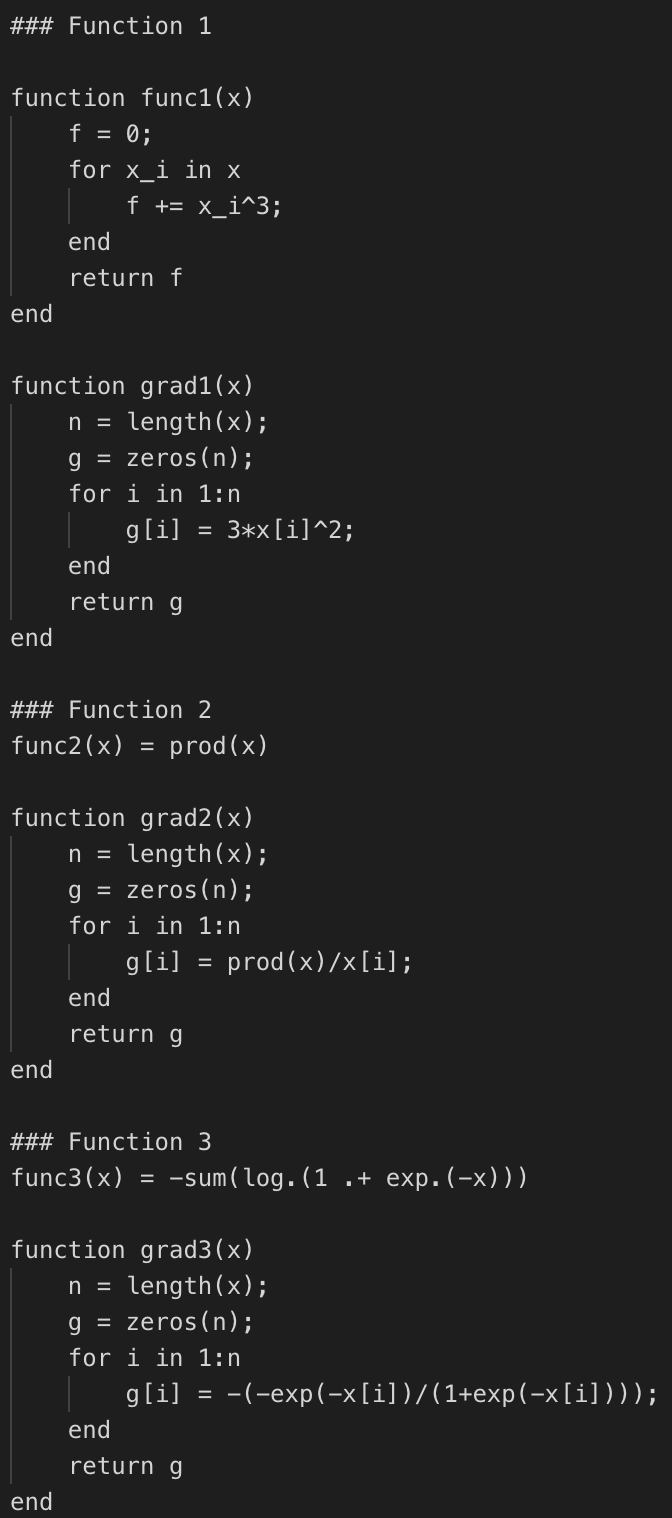
\includegraphics[width = 5cm]{DirivativeOfCode.png}

\section{Algorithms and Data Structures Review}

For these questions you may find it helpful to review these notes on big-O notation:\\
\url{http://www.cs.ubc.ca/~schmidtm/Courses/Notes/bigO.pdf}

\subsection{Trees}

\blu{Answer the following questions} You do not need to show your work.
\begin{enumerate}
\item What is the maximum number of \emph{leaves} you could have in a binary tree of depth $l$?
\ans{$2^{i}$}
\item What is the maximum number of \emph{internal nodes} (excluding leaves) you could have in a binary tree of depth $l$?
\ans{$2^{i}-1$}
\end{enumerate}
Note: we'll use the standard convention that the leaves are not included in the depth, so a tree with depth $1$ has 3 nodes with 2 leaves.


\subsection{Common Runtimes}

\blu{Answer the following questions using big-$O$ notation} You do not need to show your work.
\begin{enumerate}
\item What is the cost of running the mergesort algorithm to sort  a list of $n$ numbers?
\ans{$O(n\log n)$}
\item What is the cost of finding the third-largest element of an unsorted list of $n$ numbers?
\ans{$O(n)$}
\item What is the cost of finding the smallest element greater than 0 in a \emph{sorted} list with $n$ numbers?
\ans{$O(log n)$}
\item What is the cost of finding the value associated with a key in a hash table with $n$ numbers? \\(Assume the values and keys are both scalars.)
\ans{$O(n)$}
\item What is the cost of computing the matrix-vector product $Ax$ when $A$ is $n \times d$ and $x$ is $d \times 1$?
\ans{$O(nd)$}
\item What is the cost of computing the quadratic form $x^TAx$ when $A$ is $d \times d$ and $x$ is $d \times 1$?
\ans{$O(nd)$}
\item How does the answer to the previous question change if $A$ has only $z$ non-zeroes? (You can assume $z \geq d$)
\ans{$O(zd)$}
\end{enumerate}

\subsection{Running times of code}

Included in \texttt{a1.zip} is file named \texttt{bigO.jl}, which defines several functions
that take an integer argument $n$. For each function, \blu{state the running time as a function of $n$, using big-O notation}.
\ans{func1: $O(n)$}
\ans{func2: $O(1)$}
\ans{func3: $O(n)$}
\ans{func4: $O(n^2)$}


\section{Summary Statistics and Data Visualization}

The file \emph{a1.zip} contains estimates of the influenza-like illness percentage over 52 weeks on 2005-06 by Google Flu Trends in a comma-separated values (CSV) file. You can open this with Excel or other spreadsheet programs; the first row gives the abbreviation of the region names for each column, and each row gives the estimate for a week.
After you change to the a0 directory, you can load this data in Julia using:
\begin{verbatim}
using DelimitedFiles
dataTable = readdlm("fluTrends.csv",',')
\end{verbatim}
This creates an two-dimensional array of type ``Any''  populated with all the information in the CSV file.

\subsection{Summary Statistics}

\blu{Report the following statistics}: the minimum, maximum, mean, median, and mode of all values across the dataset. In light of thea above, \blu{is the mode a reliable estimate of the most ``common" value? Describe another way we could give a meaningful ``mode" measurement for this (continuous) data.}
\ans{Min value = 0.352\\Max value = 4.862\\ Mean = 4.862\\
Median = 1.1589999999999998 \\ Mode = 0.77\\
A more meaningful Mode can be obtained by setting intervals and count the most common intervals that values lands.
}

Hint: Since the first row of the CSV file is just the names of the columns, we can create a matrix $X$ containing the data stored as real numbers using:
\begin{verbatim}
X = real(dataTable[2:end,:])
\end{verbatim}
You can make Julia dispaly the matrix $X$ using
\begin{verbatim}
@show X
\end{verbatim}
The \emph{show} macro can be used to display the result of any expression, like showing the tenth row of $X$:
\begin{verbatim}
@show X[10,:]
\end{verbatim}
Note that this can be run inside functions, so it's helpful for debugging.

Julia has a mean and median function available, if you include the Statistics package. This package does not have a mode command, so I've included one in `misc.jl'.


\subsection{Data Visualization}

Consider the figure on the next page.
The figure contains the following plots, in a shuffled order:
\enum{
\item A histogram showing the distribution of all values in the matrix $X$.
\item A boxplot grouping data by weeks, showing the distribution across regions for each week.
\item A scatterplot between the two regions with highest correlation.
\item A single histogram showing the distribution of \emph{each} column in $X$.
\item A scatterplot between the two regions with lowest correlation.
\item A plot containing the weeks on the $x$-axis and the percentages for each region on the $y$-axis.
}
\blu{Match the plots (labeled A-F) with the descriptions above (labeled 1-6), with an extremely brief (a few words is fine) explanation for each decision.}
\ans{
    B-2 : Only boxplot.\\
    3-F : The correlation of the two values is higher than E.\\
    5-E : The correlation of the two values is lower than F.\\
    6-A : The name of the Axis matches the Disctiption.\\
    4-D : In the margin, it shows the names of each column. \\
    1-C : Only one class, which repersents all values in X.\\
}
Hint: you can generate similar plots by adding the PyPlot package. To add this package use:
\begin{verbatim}
using Pkg # Loads the package manager
Pkg.add("PyPlot") # Only needs to be done once  (installs a Julia-callable Python build)
using PyPlot # Do this once per session
plot(1:52,X[:,1]) # Plot the first row
\end{verbatim}
To generate similar-looking plots you can use the functions `plot', `boxplot', `plt.hist', and `scatter'.


\subsection{Decision Surfaces}

Consider the figure below, which plots a set of two-dimensional training examples and the decision surface produced by a ``neural network'' classifier (a model we'll see later in the course).
\blu{How many training examples has the neural network mis-classified?} (This figure is best viewed in colour.)
\ans{17}

\section{Decision Trees}

If you run the file \emph{example\_decisionStump.jl}, it will load a dataset containing longtitude and latitude data for 400 cities in the US, along with a class label indicating whether they were a ``red" state or a ``blue" state in the 2012 election.\footnote{The cities data was sampled from \url{http://simplemaps.com/static/demos/resources/us-cities/cities.csv}. The election information was collected from Wikipedia.} Specifically, the first column of the variable $X$ contains the longitude and the second variable contains the latitude, while the variable $y$ is set to $1$ for blue states and $2$ for red states. After it loads the data, it plots the data and then fits two simple classifiers: a classifier that always predicts the most common label ($1$ in this case) and a decision stump that discretizes the features (by rounding to the nearest integer) and then finds the best equality-based rule (i.e., check if a feature is \emph{equal} to some value). It reports the training error with these two classifiers, then plots the decision areas made by the decision stump. The plot should look like this:

Note that these functions use the ``JLD'' package for loading the data and the ``PyPlot'' and ``PyCall'' package to do the plotting. You can install these packages using:
\begin{verbatim}
using Pkg
Pkg.add("JLD")
Pkg.add("PyPlot")
Pkg.add("PyCall")
\end{verbatim}

\subsection{Equality vs. Inequality Splitting Rules}

In class we discussed splitting rules based on inequalities rather than equalities. \blu{Is there a type of feature where it makes sense to use 
an equality-based splitting rule?}




\subsection{Decision Stump Implementation}

The file \emph{decisionstump.jl} contains a function  that finds the best decision stump using the equality rule (``decisionStumpEquality''), and then returns a function that can apply this decision stump to new data. Instead of discretizing the data and using a rule based on testing an equality for a single feature, we want to check whether a feature is above a threshold and split the data accordingly (this is the more sane approach, which we discussed in class). \blu{Add a new function ``decisionStump'' to \emph{decision\_stump.jl} that finds the best inequality-based rule, and report the updated error you obtain by using inequalities instead of discretizing and testing equality.}

Hint: you may want to start by copy/pasting the contents of of the ``decisionStumpEquality'' function and then make modifications from there. Note that you should remove the calls to the ``round'' function for the inequality case.  Make sure that you maintain the same input/output format in your function, since otherwise subsequent questions will not work (it should produce a plot that divides the US into a northern blue and a southern red area).
If you are new to Julia, you may also want to look at\emph{majorityPredictor.jl} to get an idea of the syntax in  a simpler case.

\subsection{Constructing Decision Trees}

Once your \emph{decisionStump} function is finished, the script \emph{example\_decisionTree} will be able to fit a decision tree of depth 2 to the same dataset (which results in a lower training error). Look at how the decision tree is stored and how the (recursive) \emph{predict} function works. \blu{Using the same splits as the fitted depth-2 decision tree, write out what an alternate version of the predict function would be for classifying one training example as a simple program using if/else statements (as in the first slide of L3 that has the title ``Decision Trees'').}

Hint: you can use use the ``@show'' macro to print the values of various expressions during the execution of a .jl file.

\subsection{Cost of Fitting Decision Trees}

In class, we discussed how in general the decision stump minimizing the classification error can be found in $O(nd\log n)$ time. Using the greedy recursive splitting procedure, \blu{what is the total cost of fitting a decision tree of depth $m$ in terms of $n$, $d$, and $m$?} 

Hint: even thought there could be $(2^m-1)$ decision stumps, keep in mind not every stump will need to go through every example. Note also that we stop growing the decision tree if a node has no examples, so we may not even need to do anything for many of the $(2^m-1)$ decision stumps.

\vspace{25pt}
\textbf{HAVE YOU DOUBLE CHECKED THAT YOU'RE FOLLOWING ALL THE ASSIGNMENT SUBMISSION INSTRUCTIONS???}\\
\url{www.cs.ubc.ca/~schmidtm/Courses/340-F19/assignments.pdf}

\end{document}